\chapter{Train Benchmark Implementation}

In this chapter, we discuss the implementation details of the Train Benchmark.

\section{Performance Benchmark Framework}

\begin{figure}[!Htb]
	\centering
	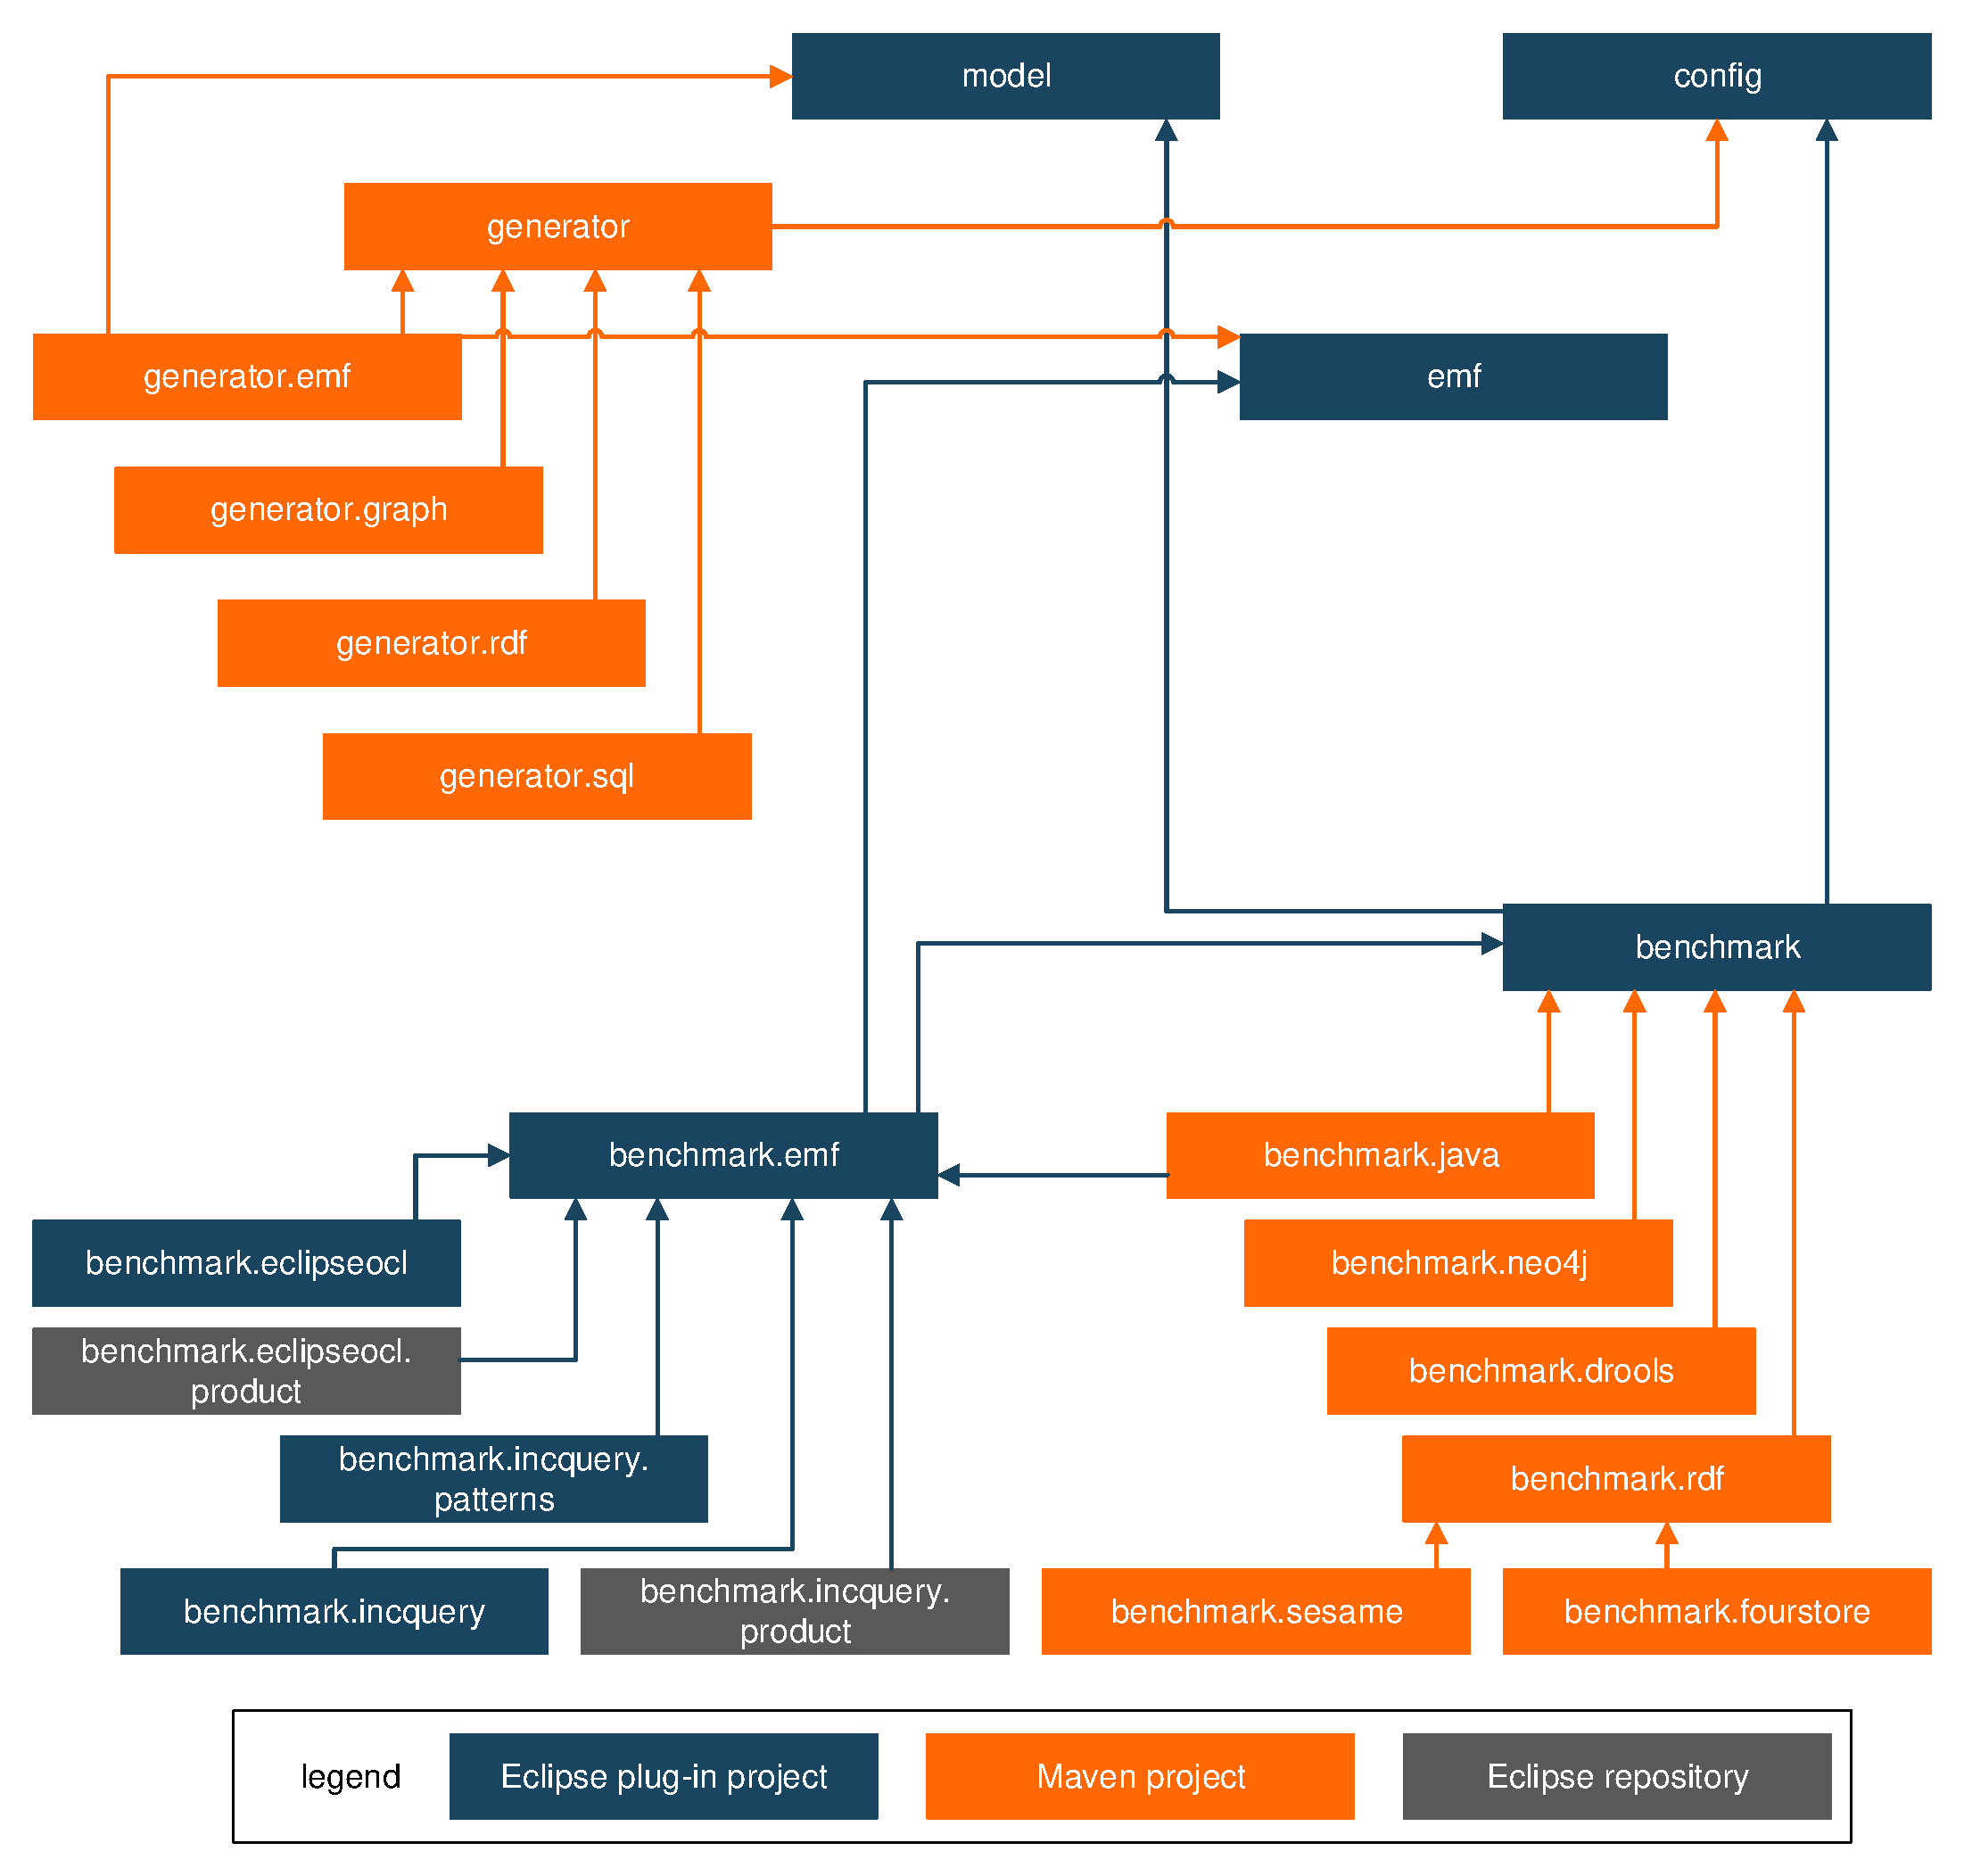
\includegraphics[width=\textwidth]{figures/trainbenchmark-modules}
	\caption{The Maven modules defined in the Train Benchmark. Note that artifact ids of the modules are shortened and the full ids start with \texttt{hu.bme.mit.trainbenchmark}.}
	\label{fig:trainbenchmark-modules}
\end{figure}

\subsection{Architecture}

For the integration of the Train Benchmark projects and their third party dependencies, we use Apache Maven~\cite{Maven}. The dependencies are shown in \figref{fig:trainbenchmark-modules}.

In this section, we briefly describe the tasks and responsibilities of each module.

\subsubsection{Parent module}

The \texttt{hu.bme.mit.trainbenchmark} module is the parent module which contains the modules used in the Train Benchmark. Building this Maven module builds all child modules as well.

\subsubsection{Central modules}

The \texttt{hu.bme.mit.trainbenchmark.model} module contains the reference metamodel represented in EMF.

\paragraph{Opening EMF instance models.} If you would like to view the EMF instance models, right click the \texttt{hu.bme.mit.trainbenchmark.model} project and choose \textbf{Run As} | \textbf{Eclipse Application}) to start a new runtime Eclipse. Import the \texttt{hu.bme.mit.trainbenchmark.instancemodels} project. The \texttt{concept} files can be opened with the \textbf{Sample Reflective Model Editor}. (Warning: opening large models may cause the Eclipse instance to hang up for a long time.) If you also wish to generate an editor, open the \texttt{models/Metamodel.genmodel} file. Right click the \textsf{Metamodel} root element and choose \textbf{Generate All}. Start a new runtime Eclipse. The \textsf{concept} files are now opened by the \textbf{Concept Editor}.

The \texttt{hu.bme.mit.trainbenchmark.config} module contains classes and constants used by the \texttt{generator} and the \texttt{benchmark} projects.


\subsubsection{Representation-specific modules}

The \texttt{hu.bme.mit.trainbenchmark.emf} and \texttt{hu.bme.mit.trainbenchmark.rdf} modules contain classes and constants used by the particular representations.



\subsubsection{Generator modules}

The \texttt{hu.bme.mit.trainbenchmark.generator.*} modules are responsible for generating the instance models for the benchmarks.

\begin{itemize}
  \item \texttt{emf}: generates an EMF instance model.
  \item \texttt{graph}: generates a property graph model in the specified format: GraphML (default), Blueprints GraphSON, Faunus GraphSON.
  \item \texttt{rdf}: generates an RDF instance model.
  \item \texttt{sql}: generates an SQL script which creates and loads the appropriate database tables.
\end{itemize}



\subsubsection{Benchmark modules}

The \texttt{hu.bme.mit.trainbenchmark.benchmark.*} modules are responsible for benchmarking. For the list of current implementations, see \autoref{tbl:tools}.

\subsubsection{4store}

To access 4store through a graph-like API, we developed a Java client\footnote{\url{https://git.inf.mit.bme.hu/w?p=projects/bigmodel/4store-graph-client.git}, \\ clone URI: \url{git@git.inf.mit.bme.hu:projects/bigmodel/4store-graph-client.git}} with a focus on high performance.

\subsection{Program parameters}
\subsubsection{Generator}
\subsubsection{Running the benchmark}

\subsection{Extending the framework with custom tools, queries or models}
\subsubsection{Extending the model generator with new syntaxes}
\subsubsection{Adding a tool to measure performance}

\subsection{Generating diagrams automatically}
\todo{R library dependencies}

Steps to generate diagrams automatically:
\begin{enumerate}
  \item Switch to the \texttt{src/hu.bme.mit.trainbenchmark.analyze} in the mondo-trainbenchmark repository
  \item Merge the measured data into \texttt{results.txt}. The file contains one header line and multiple data records belonging to (optionally) multiple series.
  \item Modify \texttt{configs.R} to introduce a new tool (specify the name of the tool in the \texttt{results.txt} file and on the diagrams), specify the line color and the type of the tool and in the \texttt{drawtools} variable enumerate tools to be plotted.
  \item Execute the \texttt{knitIt.sh} script.
  \item Inspect the generated \texttt{plotLines.html} and \texttt{plotLines-user.html} reports.
  \item If the you want the report to be zipped in a single file, execute \texttt{packHTML.sh} that generates \texttt{tbReport.zip}.
\end{enumerate}
